 \documentclass[c]{beamer}
%\documentclass{beamer}
\listfiles

\mode<presentation>
{
  %\usetheme[deutsch,titlepage0]{KIT}
\usetheme[deutsch]{KIT}
% \usetheme{KIT}

%%  \usefonttheme{structurebold}

  \setbeamercovered{transparent}

  \setbeamertemplate{enumerate items}[circle]
  %\setbeamertemplate{enumerate items}[ball]

}
\usepackage{babel}
\date{}
%\DateText

\newlength{\Ku}
\setlength{\Ku}{1.43375pt}

\usepackage[utf8]{inputenc}
\usepackage[TS1,T1]{fontenc}
\usepackage{array}
\usepackage{multicol}
\usepackage{lipsum}
\usepackage[]{algorithm2e}
\usepackage{amsmath}
\usepackage{color}

\usenavigationsymbols
%\usenavigationsymbols[sfHhdb]
%\usenavigationsymbols[sfhHb]

\subtitle{Algorithmen I SS 14}
\author[]{Vincent Schüßler}

\AuthorTitleSep{\relax}

\institute[ITI]{Institut für Theoretische Informatik}

\TitleImage[width=\titleimagewd]{images/title}

\newlength{\tmplen}

\newcommand{\verysmall}{\fontsize{6pt}{8.6pt}\selectfont}

\title[Algorithmen I SS 14]{Tutorium 11}

\usepackage{alltt}

\TitleImage[width=\titleimagewd]{images/title02}

\begin{document}

\begin{frame}
  \maketitle
\end{frame}

\begin{frame}
	\begin{center}
		\Huge
		Mittsemesterklausur
	\end{center}
\end{frame}

\begin{frame}{Duplikaterkennung}
	\begin{itemize}
		\item Gegeben: Array der Größe $n$ mit Elementen $\in {0, \ldots, n - 1}$
		\item Gesucht: Duplikat finden in $\mathcal{O}(n)$ und \emph{in-place}
		\item Bucketsort ist \textbf{nicht} in-place
		\item Betrachte Array als Permutation, löse schrittweise Zykel auf
	\end{itemize}
\end{frame}

\begin{frame}{Urlaubsdatenbank}
	\begin{itemize}
		\item Gegeben: Paare mit ID und Urlaubstag
		\item Gesucht: IDs der Mitarbeiter mit mindestens 30 Tagen Urlaub in \emph{erwartet} $\mathcal{O}(n)$
		\item Wichtig: IDs können sehr groß werden. Array über Wertebereich wird zu groß!
		\item Lösung: Hashtabelle
		\item Gesucht (2): Tag mit maximalen Urlaubsnehmern in \emph{deterministisch} $\mathcal{O}(n)$
		\item Lösung mit Array, nur 365 Tage
	\end{itemize}
\end{frame}

\begin{frame}{Aufgabe mit Graphen}
	\begin{center}
		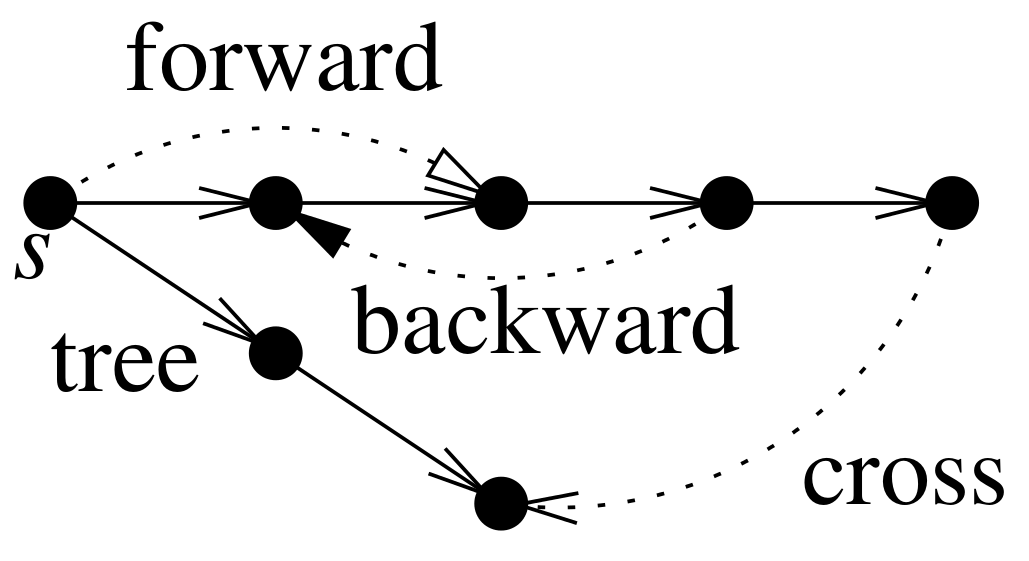
\includegraphics[keepaspectratio,scale=0.25]{images/edges}
	\end{center}
\end{frame}

\begin{frame}{Familie von Graphen}
	\begin{itemize}
		\item Familie von DAGs mit $\Omega(n^2)$ Kanten
		\item $\Omega \approx$ "`mindestens"'
	\end{itemize}
\end{frame}

\begin{frame}{Summe von Paaren}
	\begin{itemize}
		\item Gegeben: Array mit $n$ Zahlen
		\item Gesucht: $i, j$ mit $A[i] + A[j] = x$ in $\mathcal{O}(n \log{n})$
		\item Zunächst Liste sortieren
		\item Lösung 1: für jedes Element in der Liste mit binärer Suche entsprechende andere finden
		\item Lösung 2 (schneller): Bewege $i$ und $j$ vom linken bzw. rechten Rand aufeinander zu, bis Summe erreicht ist
		\item Beweis der Korrektheit, nicht Laufzeit begründen!
	\end{itemize}
\end{frame}

\begin{frame}{Aufgabe: Bottleneck Shortest Path}
	Sei $G = (V, E)$ ein zusammenhängender ungerichteter gewichteter Graph und $s, t \in V$. Ein kreisfreier Pfad P zwischen s und t heiße ein Bottleneck Shortest Path (BSP) für s und t,
	wenn das größte in P auftretende Kantengewicht minimal ist für alle Pfade zwischen s und t
	\begin{enumerate}
		\item Zeigen Sie: Ist T ein MST in G, dann ist der in T eindeutige Pfad P zwischen zwei Knoten $s, t \in V$ ein BSP in G für s und t.
		\item Geben Sie einen Algorithmus an, der für gegebenen $G = (V, E)$, gegebene $s, t \in V$ und einen gegebenen MST T in G einen BSP P zwischen s und t ausgibt.
		Die Laufzeit soll dabei in $\mathcal{O}(|P|)$ liegen.
		Nehmen Sie an T liege in Form des Array \textit{parent} vor.
		\item Argumentieren Sie kurz warum ihr Algorithmus korrekt und die geforderte Laufzeit hat.
	\end{enumerate}

\end{frame}


\begin{frame}{Kreativaufgabe: Streaming MST}
	Gegeben sei ein zusammenhängender Graph mit $n$ Knoten und $m$ Kanten.
	Die Knoten sind lokal gespeichert, während die Kanten über eine Netzwerkverbindung gestreamt werden.
	Sie können nicht lokal gespeichert werden, da nur $\mathcal{O}(n)$ Speicherplatz vorhanden ist.

	\textbf{Aufgabe 1}: Gib einen Algorithmus an, der einen MST von G unter diesen Einschränkungen bestimmt.

	\textbf{Aufgabe 2}: Verbessere diesen Algorithmus so, dass er nur $\mathcal{O}(m \log{n})$ Rechenzeit benötigt.
\end{frame}

\end{document}
